\documentclass[a4paper,cs4size]{BHCexam}
%\documentclass[a4paper,cs4size,answers]{BHCexam}

\usepackage{multicol} % 分栏
\usepackage{hyperref}
\pagestyle{fancy}
\fancyfoot[C]{\kaishu \small 第 \thepage 页 共 \pageref{lastpage} 页}
%\fancyhead[L]{\includegraphics[width=2cm]{qrcode.png}}
\title{浮力习题课}
%\subtitle{数学文科试卷}
%\notice{满分150分, 120分钟完成, \\	允许使用计算器,答案一律写在答题纸上.}
%\author{Gavin Chen}
%\date{\today}

\begin{document}
\maketitle
\begin{groups}
    \group{}

    \zihao{-4}
    \begin{questions}[]

        \question[5] 如图所示,完全相同的$a$、$b$两个长方体,长度为$h$,悬浮在密度为$\rho$的液体中,
        长方体$b$上下表面的液体压强差为\underline{\quad\quad\quad\quad}。
        若两长方体$a$、$b$下表面所受液体的压力分别为$F_a$、$F_b$,则$F_a$\underline{\quad\quad}$F_b$(选填“大于”,“等于”或
        “小于”)
        \begin{figure}[htb]
            \flushright
            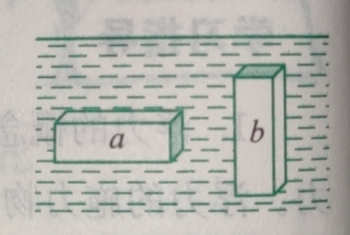
\includegraphics [scale=0.5,trim=0 0 0 0]{./image/pyhsics_buoyantforce_1.png}
            % \caption{图名}
            \label{fig:fig_buoyantforce_1.png}
        \end{figure}
        \vspace{0.5cm}

        \question[5] 质量为$0.5kg$的木块漂浮在水中,木块所受的浮力为\underline{\quad\quad\quad\quad}$N$,
        跟木块漂浮在水中相比,当其漂浮在浓盐水中时($\rho_{\text{盐水}}>\rho_{\text{水}}$),
        木块所排开液体的体积\underline{\quad\quad\quad\quad},排开液体的质量\underline{\quad\quad\quad\quad}
        (选填“变大”,“不变”或 “变小”)。
        \vspace{0.5cm}

        \question[5] 甲、乙两个完全相同的杯子盛有不同浓度的盐水,将同一个鸡蛋先后放入其中。
        当鸡蛋静止时,两个杯子中液面恰好相平,鸡蛋所处的位置如图所示,则(\quad\quad\quad\quad)
        \fourchoices{鸡蛋在乙杯中受到液体的浮力较大}
        {鸡蛋在甲杯里排开液体的质量较大}
        {甲杯底部所受的液体压力较大}
        {乙杯底部所受的液体压强较大}
        \begin{figure}[htb]
            \flushright
            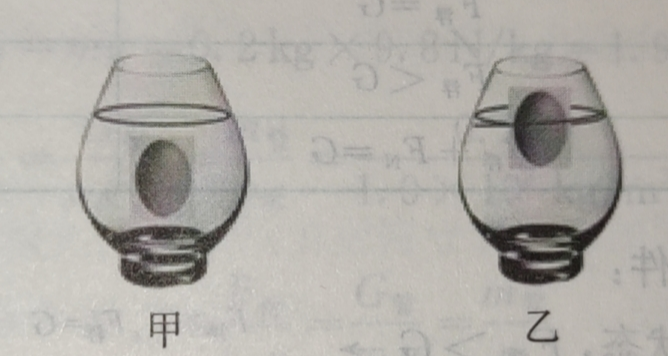
\includegraphics [scale=0.4,trim=0 0 0 0]{./image/pyhsics_buoyantforce_2.png}
            % \caption{图名}
            \label{fig:fig_buoyantforce_2.png}
        \end{figure}
        \vspace{0.5cm}

        \question[5] 如图所示,重$5.88N$的正方体木块$A$放入水中后,当其受到竖直向下的$3.92N$的压力F时,
        木块$A$恰能完全浸没在水中。求:
        \begin{subquestions}
            \subquestion 木块$A$受到的浮力。
            \subquestion 木块$A$的体积$V$。
            \subquestion 木块$A$底部受到水的压强。
            \subquestion 若去掉压力$F$,木块$A$露出水面的体积。
        \end{subquestions}
        \begin{figure}[htb]
            \flushright
            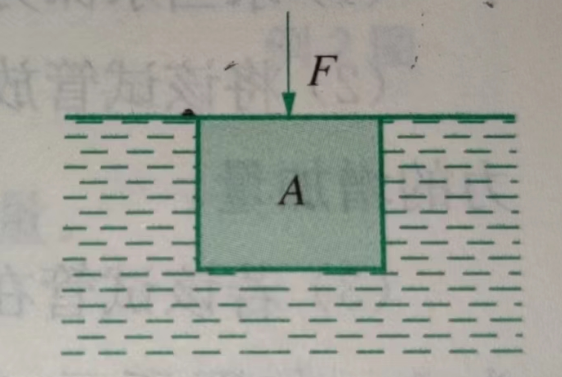
\includegraphics [scale=0.4,trim=0 0 0 0]{./image/pyhsics_buoyantforce_3.png}
            % \caption{图名}
            \label{fig:fig_buoyantforce_3.png}
        \end{figure}
        \vspace{5cm}

        \question[5] 如图所示,细线下面吊着一个体积为$100cm^3$,质量为$0.7kg$的金属块,
        当金属块浸没在底面积为$10cm^2$的柱形容器的水中时,求:
        \begin{subquestions}
            \subquestion 金属块受到的浮力。
            \subquestion 细线受到的拉力。
            \subquestion 由于金属块浸没在水中,水对容器底部的压强增加量。
        \end{subquestions}
        \begin{figure}[htb]
            \flushright
            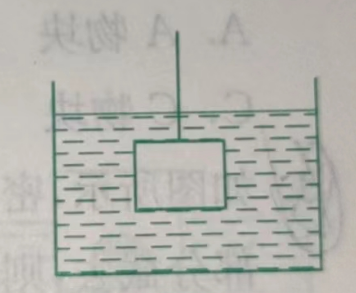
\includegraphics [scale=0.5,trim=0 0 0 0]{./image/pyhsics_buoyantforce_4.png}
            % \caption{图名}
            \label{fig:fig_buoyantforce_4.png}
        \end{figure}
        \vspace{5cm}

        \question[5] 如图所示,$A$、$B$、$C$三物块漂浮在水面上,其中密度最大的是(\quad\quad\quad\quad)
        \fourchoices{$A$物块}
        {$B$物块}
        {$C$物块}
        {无法确定}
        \begin{figure}[htb]
            \flushright
            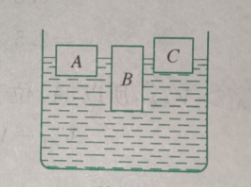
\includegraphics [scale=0.6,trim=0 0 0 0]{./image/pyhsics_buoyantforce_5.png}
            % \caption{图名}
            \label{fig:fig_buoyantforce_5.png}
        \end{figure}
        \vspace{0.5cm}


        \question[5] 如图所示,密度均匀的木块漂浮在水面上,现沿虚线将下部分截去,则剩下的部分将(\quad\quad\quad\quad)
        \fourchoices{上浮一些}
        {静止不动}
        {下沉一些}
        {无法确定}
        \begin{figure}[htb]
            \flushright
            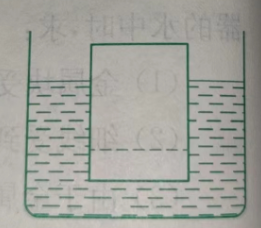
\includegraphics [scale=0.6,trim=0 0 0 0]{./image/pyhsics_buoyantforce_6.png}
            % \caption{图名}
            \label{fig:fig_buoyantforce_6.png}
        \end{figure}
        \vspace{0.5cm}


        \question[5] 浮在水面上的长方体木块的密度为$\rho$,水的密度为$\rho_0$,将木块浮在水面以上的部分切去,
        木块又会上浮,待稳定后再次切去水面以上的部分,剩余木块的体积正好是原来的$\frac{1}{2}$,求$\rho:\rho_0$。
        \vspace{5cm}

        \question[5] 如图所示,底面积为$2\times 10^{-2}m^2$的圆柱形平底薄壁水槽放在水平地面上,一装有金属球的小盆漂浮在水槽的水面上,
        小盆的质量为$1kg$,金属球的质量为$1.6kg$,金属球的体积为$0.2\times 10^{-3}m^3$。若把金属球从盆中拿出并放入水槽中,小球沉入水底。
        \begin{subquestions}
            \subquestion 求容器对水平地面压强的变化量。
            \subquestion 求水对水槽底部的压强变化量。
        \end{subquestions}
        \begin{figure}[htb]
            \flushright
            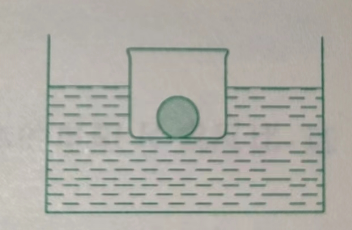
\includegraphics [scale=0.5,trim=0 0 0 0]{./image/pyhsics_buoyantforce_7.png}
            % \caption{图名}
            \label{fig:fig_buoyantforce_7.png}
        \end{figure}
        \vspace{6cm}

        \question[5] 足够高的薄壁圆柱形容器放在水平地面上,底面积为$2\times 10^{-3}m^2$,盛有质量为$0.4kg$的水。
        将一横截面积为$4\times 10^{-4}m^2$的圆柱形玻璃管,装人一定量的水后竖直放入容器中,
        玻璃管处于漂浮状态,如图中甲所示。
        \begin{subquestions}
            \subquestion 求容器内水的体积$V_{\text{水}}$。
            \subquestion 求容器中离水面$0.1m$深处的液体压强$p$。
            \subquestion 再将一实心均匀物块浸没在玻璃管的水中,玻璃管仍旧漂浮在水面上,如图中乙所示。若物块投入前后,
            管内的水对玻璃管底部压强的变化量是$\Delta p_1$,容器内的水对容器底部压强的变化量是$\Delta p_2$,
            已知$\Delta p_1=2\Delta p_2$,求物块的密度$\rho_{\text{物}}$。
        \end{subquestions}
        \begin{figure}[htb]
            \flushright
            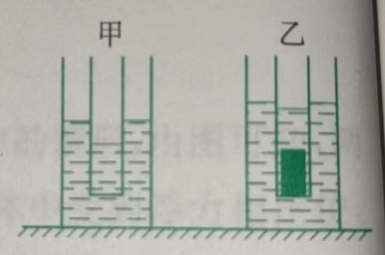
\includegraphics [scale=0.5,trim=0 0 0 0]{./image/pyhsics_buoyantforce_8.png}
            % \caption{图名}
            \label{fig:fig_buoyantforce_8.png}
        \end{figure}





    \end{questions}
\end{groups}


\label{lastpage}
\end{document}
